\documentclass[xcolor=dvipsnames]{beamer}
\usetheme{Hannover}
\usecolortheme[light]{solarized}
\usepackage{tikz}
\title{ExplainShell for Chrome}
\author{{\bf Justin Gallagher, Ted Li},\\ Jacob Zimmerman, Howard Chen}
\institute{Carnegie Mellon University}
\date{\today}
\setbeamertemplate{caption}[numbered]
\makeatletter
\def\parsecomma#1,#2\endparsecomma{\def\page@x{#1}\def\page@y{#2}}
\tikzdeclarecoordinatesystem{page}{
    \parsecomma#1\endparsecomma
    \pgfpointanchor{current page}{north east}
    % Save the upper right corner
    \pgf@xc=\pgf@x%
    \pgf@yc=\pgf@y%
    % save the lower left corner
    \pgfpointanchor{current page}{south west}
    \pgf@xb=\pgf@x%
    \pgf@yb=\pgf@y%
    % Transform to the correct placement
    \pgfmathparse{(\pgf@xc-\pgf@xb)/2.*\page@x+(\pgf@xc+\pgf@xb)/2.}
    \expandafter\pgf@x\expandafter=\pgfmathresult pt
    \pgfmathparse{(\pgf@yc-\pgf@yb)/2.*\page@y+(\pgf@yc+\pgf@yb)/2.}
    \expandafter\pgf@y\expandafter=\pgfmathresult pt
}
\makeatother

\begin{document}

\begin{frame}
\titlepage
\end{frame}

\begin{frame}{Table of Contents}
  \tableofcontents
\end{frame}

\section{Project Overview}\label{project-overview}
\begin{frame}{Project Overview}
\begin{itemize}
\itemsep8pt\parskip0pt\parsep0pt
\item
  Chrome extension to provide easy lookup of bash commands using
  \href{http://www.explainshell.com/}{explainshell.com}
\item
  Backend analytics site to show trending commands, referring sites,
  popular pages, etc.
\end{itemize}
\end{frame}

\section{Rationale}\label{rationale}
\begin{frame}{Rationale Behind
ExplainShell}
\begin{itemize}
\itemsep5pt\parskip0pt\parsep0pt
\item
  Random bash commands found online pose threat to unsuspecting users

  \begin{itemize}
  \itemsep3pt\parskip0pt\parsep0pt
  \item
    people have a risk of running malicious or insecure commands
  \end{itemize}
  \pause
\item
  Often difficult to look through \texttt{man} pages for bash command
  usage
  \begin{itemize}
  \itemsep5pt\parskip0pt\parsep0pt
  \item
    ExplainShell for Chrome attempts to reduce the effort of lookup to bare minimum
  \end{itemize}
  \pause
\item
  Helps users discover and explore more bash commands
\end{itemize}
\end{frame}


\section{Goals}\label{goals}
\begin{frame}{Goals}
\begin{itemize}
\itemsep5pt\parskip0pt\parsep0pt
\item<1->
  Develop Chrome Extension that identifies and extracts bash commands
  from web pages

  \begin{itemize}
  \itemsep3pt\parskip0pt\parsep0pt
  \item<1->
    Add a link to each bash command that redirects users to the usage
    explanation on \href{http://www.explainshell.com/}{explainshell.com}
  \item<1->
    Display friendly in-page popup of command usage when users hover
    over a bash command
  \end{itemize}
\item<2->
  Develop backend analytics site to keep track of bash commands that
  users lookup

  \begin{itemize}
  \itemsep3pt\parskip0pt\parsep0pt
  \item<2->
    Provides analytics based on what commands are being searched for
  \item<2->
    Helps users explore and discover commands they are not familiar with
  \end{itemize}
\item<3->
  Contribute to ExplainShell API
\item<4->
  Eventually publish on Chrome Web Store for people to use
\end{itemize}
\end{frame}

\section{Approach}\label{approach}
\begin{frame}{Technologies Used}
\begin{itemize}
\itemsep5pt\parskip0pt\parsep0pt
\item
  Chrome Extension: HTML/CSS/Javascript
\item
  Backend analytics site: Node.js
\item
  VC with Git (on \href{gitrepo}{Github})
\end{itemize}
\end{frame}

\begin{frame}{Approach}
\begin{enumerate}
\def\labelenumi{\arabic{enumi}.}
\itemsep6pt\parskip0pt\parsep0pt
\item<1->
  Rudimentary version of Chrome extension: Allow users to select text
  and lookup selected command.
  \only<2>{
    \begin{tikzpicture}[remember picture,overlay]
    \node at (page cs:0.1,-0.25) 
      {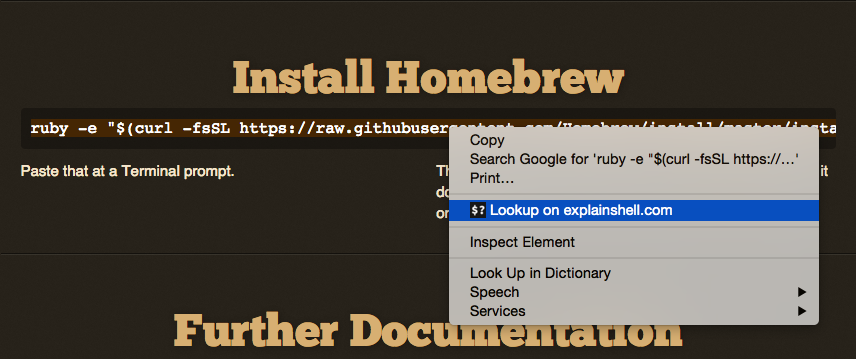
\includegraphics[width=.9\textwidth]{lookup.png}};
    \end{tikzpicture}}
\item<4->
  Develop heuristics to identify and extract bash commands automatically
  from a web page
\item<5->
  In-page link to jump to explainshell.com
  \only<6>{
    \begin{tikzpicture}[remember picture,overlay]
    \node at (page cs:0.05,-0.375) 
      {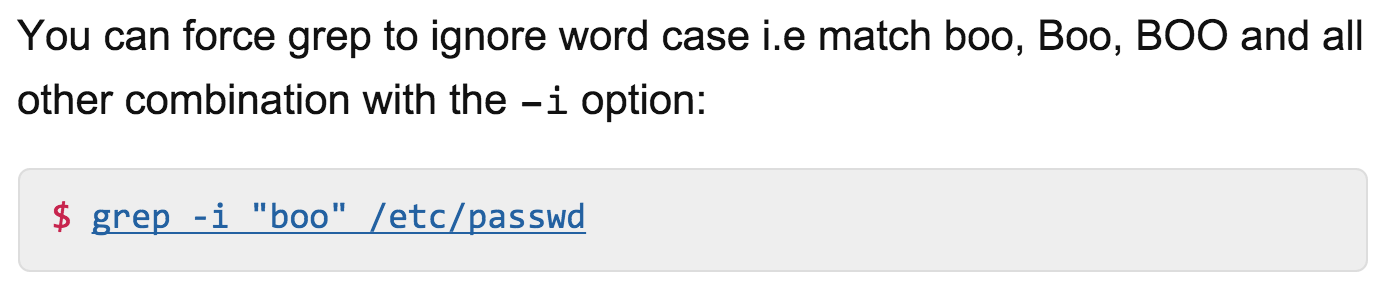
\includegraphics[width=.8\textwidth]{mode1.png}};
    \end{tikzpicture}}
\item<8->
  Insert in-page summary on hover
  \only<9>{
    \begin{tikzpicture}[remember picture,overlay]
    \node at (page cs:0.15,0) 
      {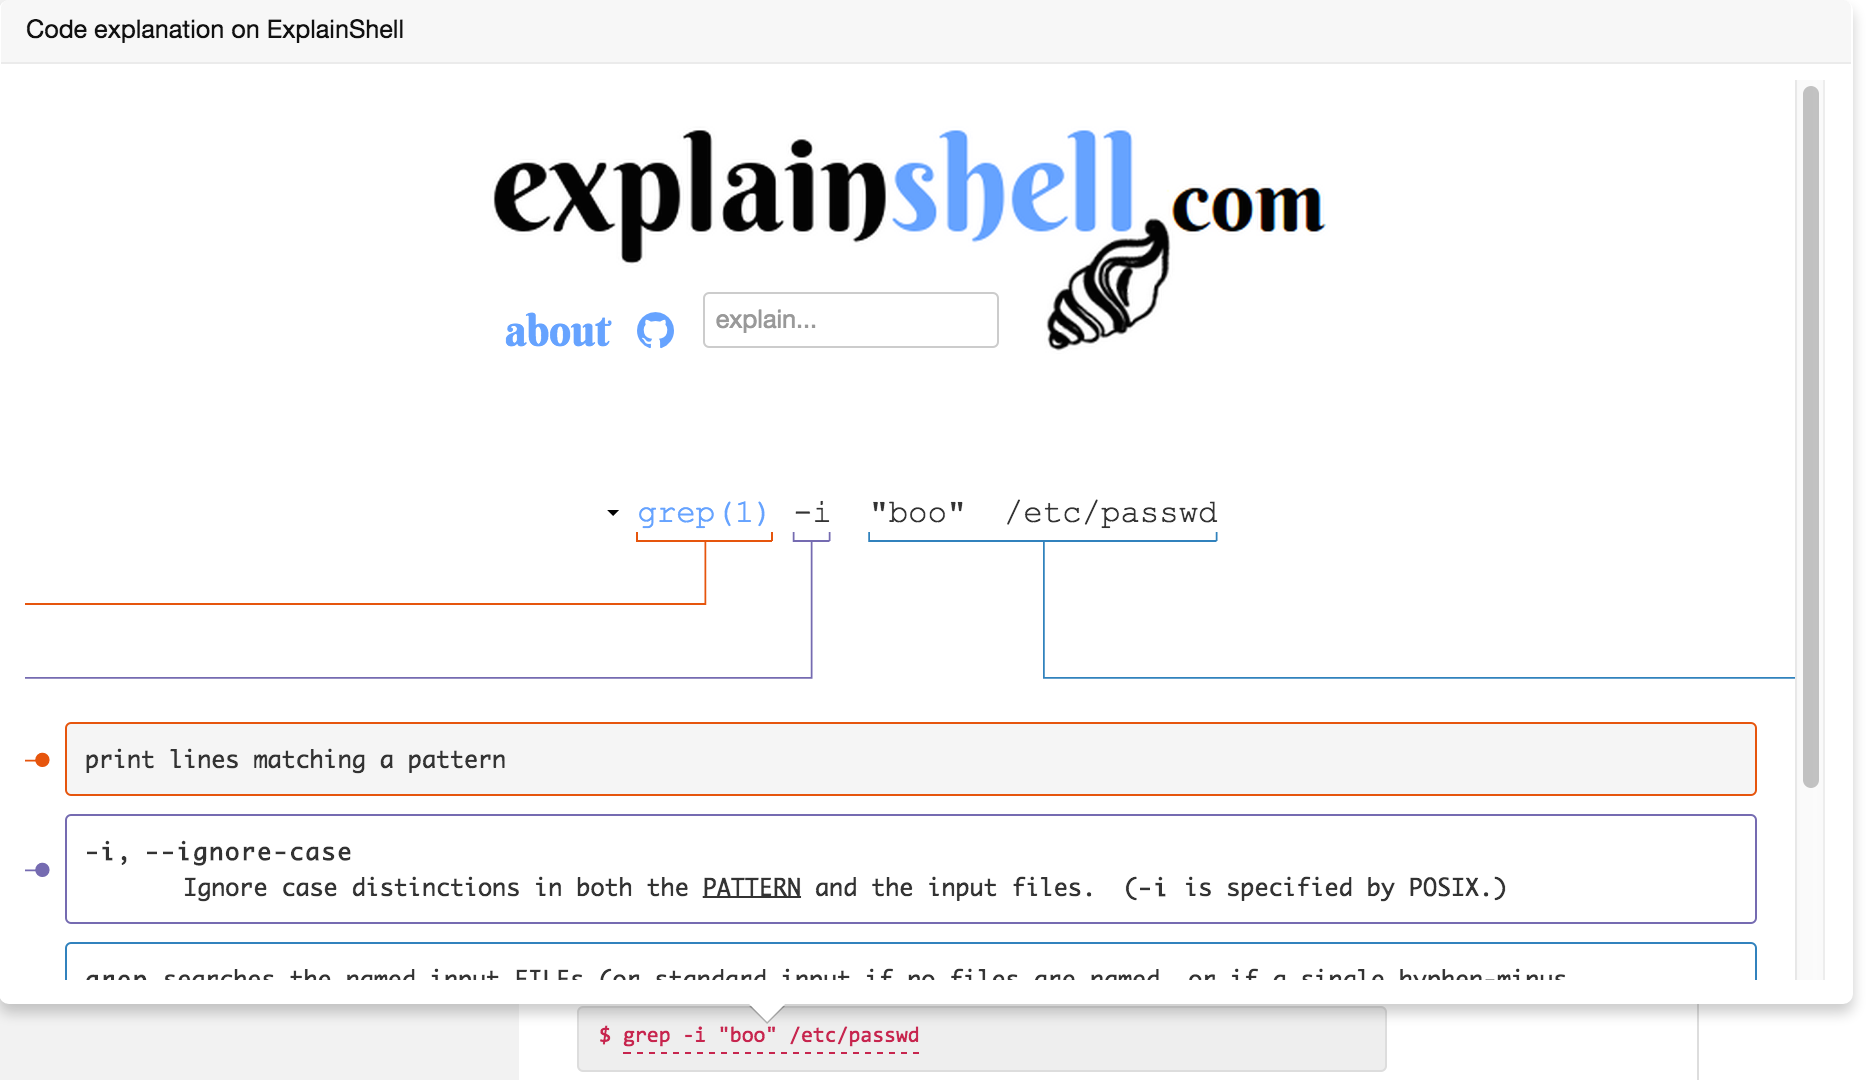
\includegraphics[width=\textwidth]{mode2.png}};
    \end{tikzpicture}}
\item<11->
  Develop backend analytics site
\item<12->
  Integrate analytics site with Chrome extension
\end{enumerate}
\end{frame}


\section{Schedule}\label{schedule}
\begin{frame}{Original Schedule}
\begin{figure}[h]
  \vspace*{-2em}
  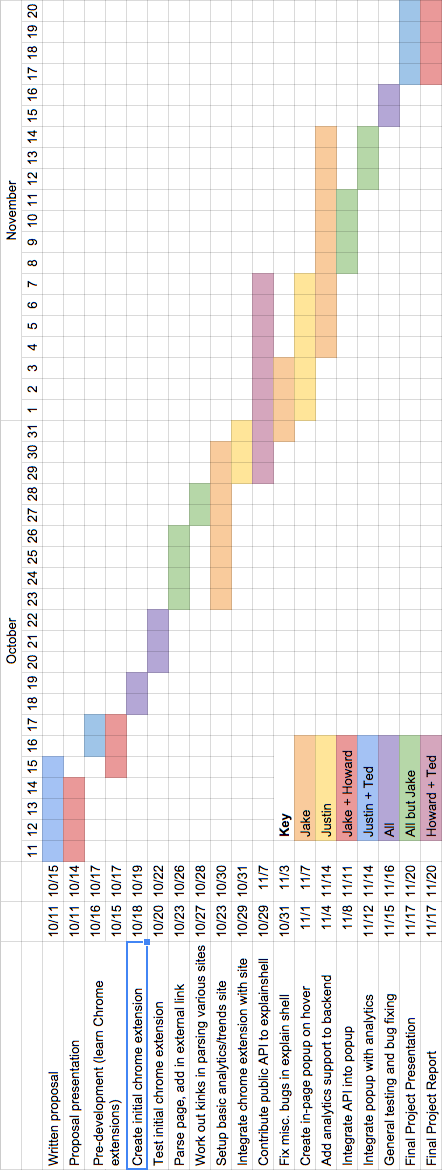
\includegraphics[width=.38\textwidth, angle=-90]{gantt-chart-rotated.png}
  \caption{\small Gantt Chart of original plan\label{gantt-chart-org}}
\end{figure}
\end{frame}

\begin{frame}{Revised Schedule}
\begin{figure}[h]
  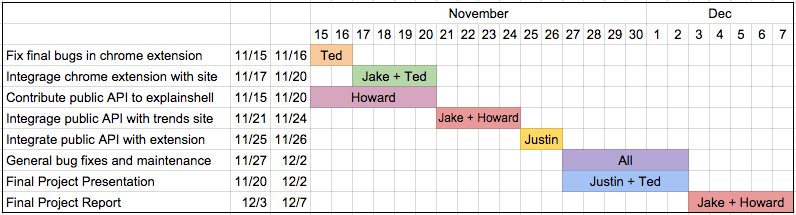
\includegraphics[width=\textwidth]{gantt-chart-revised-only.png}
  \caption{\small Gantt Chart of revised plan\label{gantt-chart-rev}}
\end{figure}
\end{frame}


\section{Results}\label{results}
\begin{frame}{Results}
\begin{itemize}
\itemsep1pt\parskip0pt\parsep0pt
\item
  Chrome extension supports embedded links and popups

  \begin{itemize}
  \itemsep1pt\parskip0pt\parsep0pt
  \item
    Still no public API for explainshell.com
  \item
    Popups pull up the full explainshell website
  \item
    HTTPS not supported
  \item
    Reports correctly to the trends website
  \end{itemize}

\pause
\item
  Fully functional trends website

  \begin{itemize}
  \itemsep1pt\parskip0pt\parsep0pt
  \item
    Track number of uses of extension
  \item
    View clicks by time, source page, domain, and command
  \item
    No authentication, API call in plain text Javascript
  \end{itemize}
\end{itemize}
\end{frame}


\section{Lessons Learned}\label{lessons-learned}
\begin{frame}{Lessons Learned}
\begin{itemize}
\itemsep1pt\parskip0pt\parsep0pt
\item
  Plan lots of extra time to accommodate for changing schedules

  \begin{itemize}
  \itemsep1pt\parskip0pt\parsep0pt
  \item
    We were often behind deadlines, causing others to be held up by
    bottlenecks
  \item
    Keep people accountable to deadlines
  \end{itemize}

\pause
\item
  Contributing to open source software is a large undertaking

  \begin{itemize}
  \itemsep1pt\parskip0pt\parsep0pt
  \item
    Need to read lots of documentation and unfamiliar code
  \item
    Pull requests take time
  \item
    A lot of work is necessary to do it properly
  \end{itemize}

\pause
\item
  Documenting your code is essential

  \begin{itemize}
  \itemsep1pt\parskip0pt\parsep0pt
  \item
    We often had problems running each others' code
  \item
    Time is wasted trying to decipher what code is doing rather than
    adding to it
  \end{itemize}
\end{itemize}
\end{frame}


\section{Summary}\label{summary}
\begin{frame}{Summary}
\tableofcontents
\end{frame}


\section{Demo}\label{demo}
\begin{frame}{Demo}
\begin{figure}[h]
  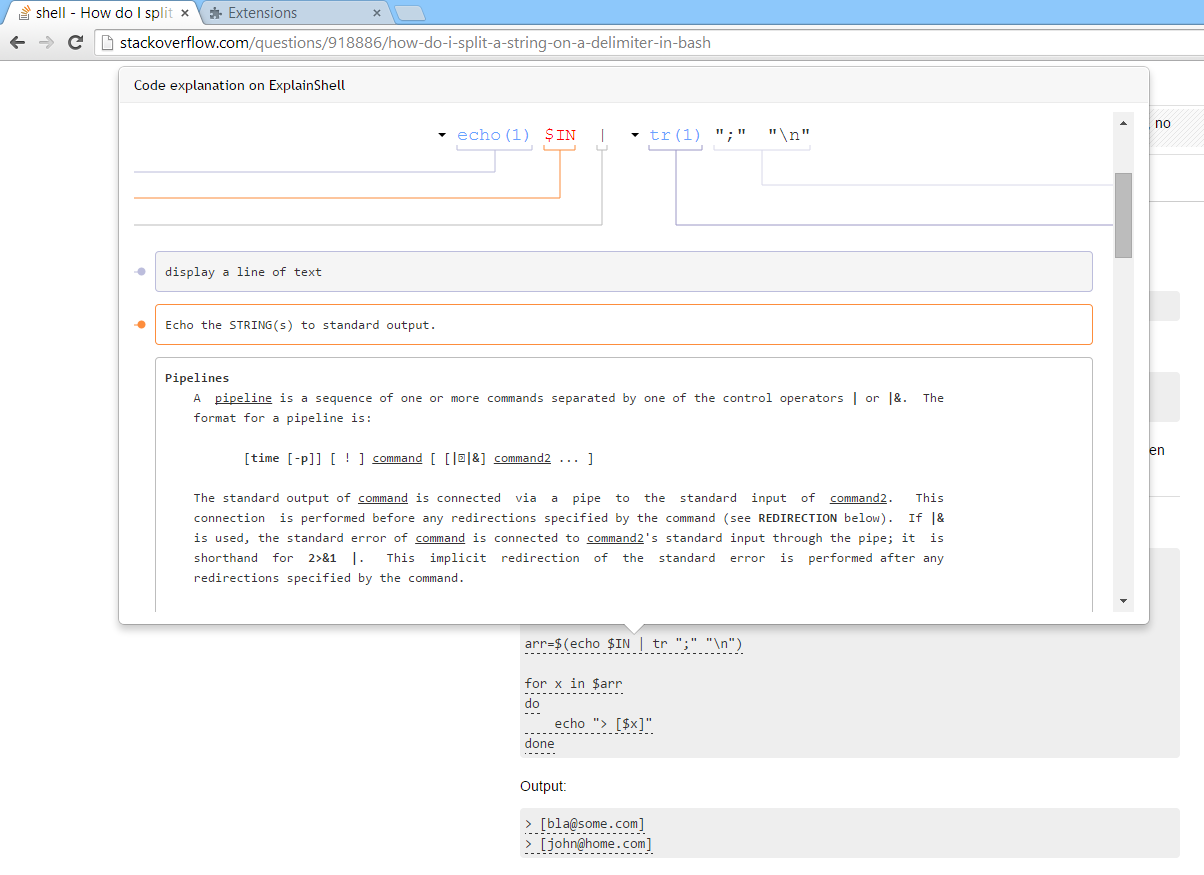
\includegraphics[width=.8\textwidth]{screenshot.png}
  \caption{Screenshot of ExplainShell Chrome Extension}
\end{figure}
\end{frame}

\end{document}